\documentclass{article}

\usepackage{hyperref}
\usepackage{lipsum}
\usepackage{circuitikz}
\usepackage{graphicx}
\usepackage[margin=0.9in]{geometry}
\usepackage{setspace}
\usepackage{mathtools}
\newtagform{brackets}{[}{]}
\usetagform{brackets}

\title{Capacitance and Optics, Lab 2}
\author{Bijan Varjavand, Khalid Elawad, Austin Wilson}
\date{March 14 2017}
\begin{document}
\maketitle
\vspace{4.5 in}
\section*{Abstract}
\ \ \ This lab compared the results of many different experiments, each measuring a variety of electrical and optical properties. The first experiment averaged the dielectric constant for 3 materials across 3 frequencies, resulting in dielectric constants of 5.58 for ceramic, 8.83 for glass, and 5.41 for firebrick. These values have a percent deviation of 43, 91.1, and 11.3 from literature values of 9.8, 4.6, and 6.1. The next experiment measured the dielectric constant of different ionic environments of firebrick at 5 frequencies - showing that increasing frequency decreased capacitance. The next part of the lab, more closely related to optical properties, investigated the efficiency of light propagation through a tube based on different wavelengths, tube lengths, and waveguide interfaces. It was seen that total internal reflection occurred most frequently at low-angle interfaces with an appropriate difference in refractive index at the interface. It was also seen that signal loss occurs steadily over distance, and that our commercial waveguide behaves poorly for infrared light. It was also shown that a material can become less visible when submerged in solution of similar refractive index.


\clearpage
\onehalfspacing
\section*{Introduction}
\ \ \ Understanding of the electronic properties of materials is critical as a material scientist. This lab specifically focused on the material properties related to capacitance and optics. These two concepts have far-reaching implications in the real world, from data and energy transfer to simple RC circuits. The purpose of this lab is broken up into 3 distinct categories. The first is to use an LCR meter (inductance, capacitance, and resistance) to measure the capacitance of copper across different dielectrics at different frequencies. We then use this data to calculate the dielectric coefficient of each material, explained later in this introduction. The next section deals with optics, as we qualitatively compare indices of refraction between two materials based on how well they bend light continuously together. The last section was to observe the phenomenon of light traveling through a waveguide to understand how total internal reflection behaves.
\subsubsection*{Parallel-Plate Capacitors in a Vacuum}
\ \ \ Due to their ability to store electrical potential difference, capacitors are one of the most critical components in a circuit. Capacitors are also able to be used with each other in circuits, in series or parallel. In series, the inverse of each capacitance is summed, while in parallel the capacitances are simply summed. This is due to the increase in surface area for potential difference for capacitors. Their applications include energy storage and the suppression of voltage spikes. In our investigation, we focus on the electrical properties of parallel-plate capacitors containing a dielectric material. This type of capacitor consist of two conductive plates with an area, A, separated by a distance, D. The capacity of a capacitor to store charge is known as its capacitance, defined by \textbf{Equation 1} below.
\begin{equation}
C = \frac{Q}{V}
\end{equation}
Capacitance, C, is thus defined by the ratio of the quantity of charge stored on any plate, Q, over a voltage across the capacitor, V. This can be though of intuitively as how much charge a single volt will supply the capacitor with. Capacitance is not usually so easily calculated, due to the presence of materials separating the two parallel plates. The simple way to approach capacitance is to first understand the behavior of a capacitor with a vacuum separating the plates. This is given by \textbf{Equation 2} below.
\begin{equation}
C = \varepsilon_0\frac{A}{D}
\end{equation}
Here we have the variables described above for parallel-plate capacitors, with the addition of an $\varepsilon_0$. This is known as the permittivity of free space (in a vaccuum), equal to $8.854x10^{-12}\frac{F}{m}$. This is intuitively understood as the reduction of potential difference across a capacitor.
\subsubsection*{Addition of a Dielectric}
\ \ \ The inclusion of a dielectric material between parallel-plate capacitors is significant in its effect on the electronic properties of a capacitor. In order for a material to be a dielectric, it must be electrically insulating and must exhibit an electric dipole structure under an applied electric field. A good way to think about the effect of the dielectric is by understanding its relative permittivity, $\varepsilon_r$, shown in \textbf{Equation 3}.
\begin{equation}
\varepsilon_r = \frac{\varepsilon}{\varepsilon_0}
\end{equation}
It can be seen by this equation that the relative permittivity of a material is simply how well it permits a potential difference between two charged plates compared to a vacuum. This is also known as the dielectric constant. This changes our \textbf{Equation 2} for a more accurate value of capacitance with a known dielectric material.
\begin{equation}
C = \varepsilon_r\varepsilon_0\frac{A}{D}
\end{equation}
It can be seen that the relative permittivity of a material will always be greater than 1, since any material has a higher permittivity than that of a vacuum. This is illustrated by \textbf{Figure 1} below.
\begin{figure}[h!]
	\begin{minipage}{.5\textwidth}
		\centering
		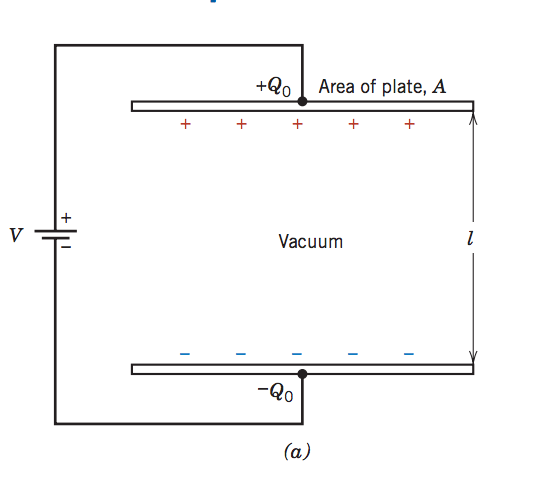
\includegraphics[width=.7\linewidth]{cap.png}
	\end{minipage}
	\begin{minipage}{.5\textwidth}
		\centering
		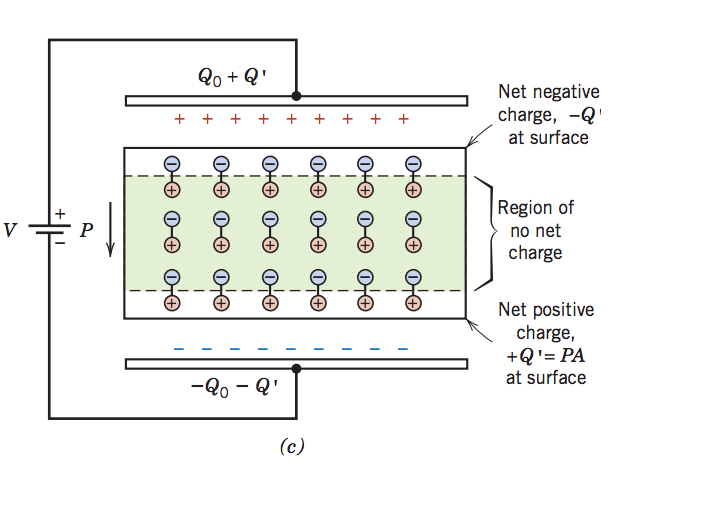
\includegraphics[width=.87\linewidth]{cap_vacuum.png}
	\end{minipage}
	\caption{Parallel-plate capacitors separated by a) a vacuum and b) a dielectric}
\end{figure}

\textbf{Figure 1} clearly shows how the addition of any material, no matter its permittivity, will allow for more permittivity than with a vacuum. This increase is caused by increased polarization within the material. Further, when an electric field is applied to a dielectric material the dipole moments within the material become mutually aligned, thus polarizing the material \textbf{Figure 1}. Because of this polarization, the charge density on the plates for the capacitor increases, reducing the effects of the electric field on the capacitor. In other words, the net accumulation of negative and positive charge on opposite sides of the capacitor at the surface of the dielectric is increased.

\subsubsection*{Polarization of a Dielectric}
\ \ \ There are three types of polarization that can cause a material to be a dielectric: electronic polarization, ionic polarization, and orientation polarization. Electronic polarization occurs in all dielectric materials. It occurs when the negatively charged electron cloud is displaced from the positively charged nucleus by an electric field, shown in \textbf{Figure 2}. Ionic polarization occurs when the applied field causes cations and anions to displace in opposite directions creating a net dipole movement, also in \textbf{Figure 2}. Finally, orientation polarization occurs when a material contains dipole moments in the absence of an electric field and these dipoles rotate in the presence in an electric field, also in \textbf{Figure 2}. The total polarization of a material is the sum of the three types of polarization within a material, shown below.
\begin{figure}[h!]
	\begin{minipage}{.33\textwidth}
		\centering
		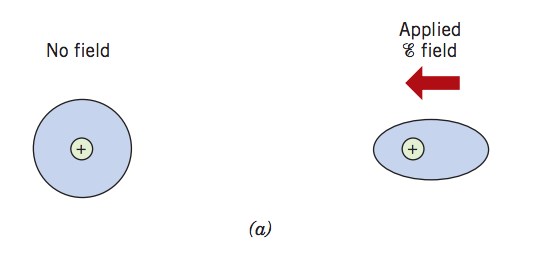
\includegraphics[width=\linewidth]{electric.png}
	\end{minipage}
	\begin{minipage}{.33\textwidth}
		\centering
		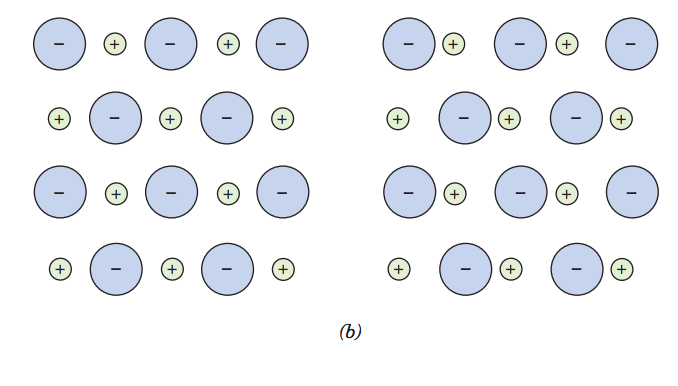
\includegraphics[width=\linewidth]{ionic.png}
	\end{minipage}
	\begin{minipage}{.33\textwidth}
		\centering
		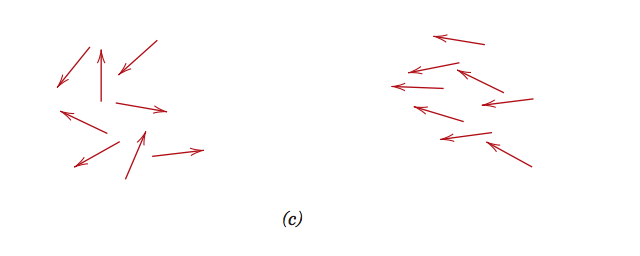
\includegraphics[width=\linewidth]{dipole.png}
	\end{minipage}
	\caption{The three types of polarization in a dielectric}
\end{figure}

\ \ \ Because the electric field changes as the direction of the current changes, when the current is alternating the degree of polarization will depend on the frequency of the current applied. When the current reverses direction, the dipoles within a dielectric material will reverse in orientation. This process of reversing orientation will take time and depend on the type of polarization present. The inverse of the minimum time taken for reorientation is know as the relaxation frequency. When the frequency of the electric field applied is greater then the relaxation frequency, the dipoles within the material will no longer have time to completely rearrange before the direction of the E field change. Thus, because of loss in polarization the E field will no longer contribute to the dielectric constant at higher frequencies.  Further as at the frequency approaches the relaxation frequency there is also an increase in the electrical energy absorbed by a material, dielectric loss. For these reasons, capacitance can therefore be thought to impede flow of AC charge carriers by storing energy as a potential difference.\\
\ \ \ Different polarization types will differ in their relation to frequency \textbf{Figure 3}. At frequencies above $10^{10}Hz$ orientation frequency will no longer play a role in the dielectric constant - suggesting that the frequency is above the frequency for a material with orientation polarization. For similar reasoning, in \textbf{Figure 3} you see that ionic polarization ceases to contribute the dielectric constant above $10^{14}Hz$. Finally, electronic polarization also loses its effect after the frequency surpasses $15^{17}Hz$ in \textbf{Figure 3}.
\begin{figure}[h!]
\centering
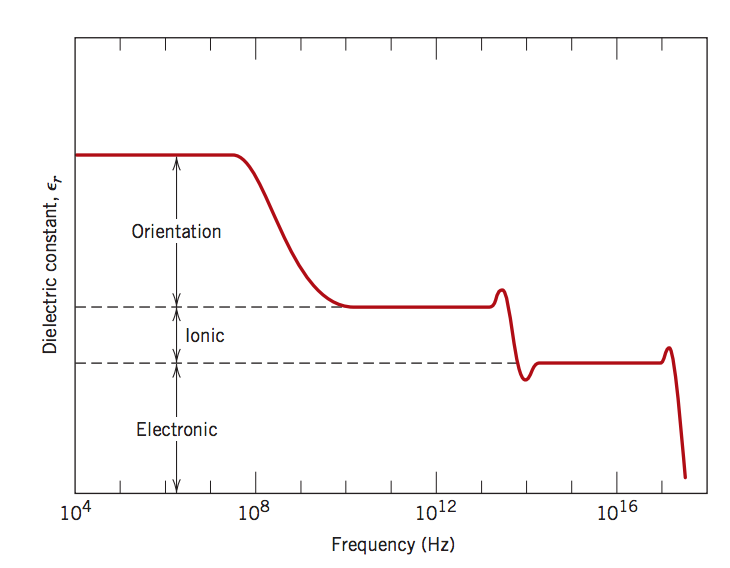
\includegraphics[scale=0.4]{polarize.png}
\caption{The components of the total polarizability of a dielectric as a function of frequency}
\end{figure}

\ \ \ Another interesting variable to note is the dissipation factor, which was measured alongside our capacitance values. This factor determines how readily a capacitor loses its polarizability. A benchmark is the value of 0 for an ideal capacitor which doesn't lose its polarizability.

\subsubsection*{Optical Properties}
\ \ \ The optical properties of a material has many intricate relationships and effects on the rest of the materials properties. For example, a material which has uniform chirality will have different optical properties that a material with alternating chirality. The relevant physical properties of materials in question with regards to optics are all dependent on the wavelength, $\lambda$, of the light. Moving further, we actually care more about the energy of each photon with a specific wavelength, given by \textbf{Equation 5} below.
\begin{equation}
E = hv
\end{equation}
Where E is the energy of the photon, $h$ is Planck's constant ($6.626x10^{-34}m^2kgs^{-1}$), and v is the frequency of the light which is just $\frac{c}{\lambda}$. The specific wavelengths explored in this part of the lab include the visual wavelengths (from $0.4-0.7\mu m$), a tiny portion of the entire spectrum ranging from $10^{-12}-10^{5}m$.\\
\ \ \ A key concept in optics is that fact that the phase velocity of light, c, is a constant $3.0x10^8\frac{m}{s}$. The behavior of light in different materials is highly dependent on the material's affect on the light's drift velocity. The drift velocity of light can be though of as how difficult it is for light to penetrate the material and pass through it. This phenomenon is described by $n$, the index of refraction of the material, given by \textbf{Equation 6}. We also include the definitions for the speed of light as a function of the electric ($\epsilon$) and magnetic ($\mu$) permeabilities.
$$c = \frac{1}{\sqrt{\epsilon_0\mu_0}}$$
$$v = \frac{1}{\sqrt{\epsilon\mu}}$$
\begin{equation}
n = \frac{c}{v} = \frac{\sqrt{\epsilon\mu}}{\epsilon_0\mu_0} = \sqrt{\epsilon_r\mu_r} = \sqrt{\epsilon_r}
\end{equation}
\ \ \ We can make the simplification in \textbf{Equation 6} since the assumption that dielectric materials will have insignificant magnetic permeabilities is a safe one. Very large indexes of refraction result in light being slowed down significantly when compared to its speed in a vacuum. It is also important to take into account the fact that light is affected by the same material differently depending on the amount of energy in the specific photons. This is how the phenomenon of refraction occurs, since the differences of energy of light in the visible spectrum (e.g. between blue and red light) result in varying effects of bending of light. This specific event of refraction of light is given by Snell's Law, shown in \textbf{Equation 7}.
\begin{equation}
n_isin\theta_i = n_esin\theta_e
\end{equation}
Here, the i and e subscripts represent the incident and exiting rays. This is because \textbf{Equation 7} represents the behavior of refraction only across a single interface. The equations shown how, depending on the differences between the refractive indices of the two materials at the interface, the light will bend varying amounts. So, a photon from a material with large n passing an interface into a material with small n, the exit angle will be smaller. This is useful when analyzing the phenomenon of total internal reflection, as once the exit angle is $90^o$ the effect of refraction is completely nullified and the material will not pass through the interface at all. The only option left for the photon is to reflect off of the interface. This phenomenon is shown below in \textbf{Figure 4}.
\begin{figure}[h!]
\centering
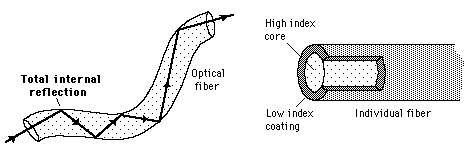
\includegraphics[scale=.8]{totalinternal.png}
\caption{The phenomenon of total internal reflection}
\end{figure}

Total internal reflection is responsible for optical fiber technology being possible, as a binary signal of light or no light can be passed through a tube with accuracy.\\

When dealing with circuits involving LEDs and phototransistors, we need to take new variables into account. These are the launch power($P_0$) and the attenuation coefficient($\alpha$). The launch power is related to the intensity of light an LED gives off, and the attenuation coefficient affects how quickly light is absorbed into a material. The relationships are shown below in \textbf{Equations 8, 9, and 10}.
\begin{equation}
P_i = P_0 e^{-\alpha l}
\end{equation}
\begin{equation}
\alpha = \frac{ln(P_1/P_2)}{L_2-L_1}
\end{equation}
\begin{equation}
\alpha = \frac{ln(I_1/I_2)}{L_2-L_1}
\end{equation}
Here, we use P, I, and L with subscripts to represent the power, current, and length exiting individual optic fibers. These relationships make intuitive sense as well, as \textbf{Equation 8} simply shows how a signal loses power over distance, \textbf{Equation 9} solves for attenuation with two measurements of length and power, and \textbf{Equation 10} does the same but with current instead of power.

\section*{Procedure}
\subsubsection*{Lab 2a}
\begin{itemize}
\item We prepared three different dielectric material samples: ceramic, glass, and firebrick and measured their thicknesses.
\item We attached copper tapes of three known areas on both sides.
\item Using an LCR meter, we measured the capacitance and dissipation factor for three measurements, each at three frequencies: 100Hz, 1kHz, and 100kHz. This was repeated for all of the copper tapes of differing areas.
\end{itemize}
\subsection*{Lab 2b}
\begin{itemize}
\item We prepared a single dielectric sample of firebrick and measured its thickness.
\item We attached three copper tape pieces of differing areas on one side, and attached a single copper tape sheet on the second side so that the areas of the pieces on the first side overlapped with the sheet on the second.
\item Using the LCR meter, we again measured three values for capacitance and dissipation factor at three different frequencies. \textit{This was done incorrectly as we needed three different frequencies, so our data for this section is from \ Maria Lugo's group.}
\end{itemize}
\subsubsection*{Lab 2c circuit}
\begin{itemize}
\item We prepared a circuit with a breadboard as shown in \textbf{Figure 5}
\begin{figure}[h!]
	\centering
	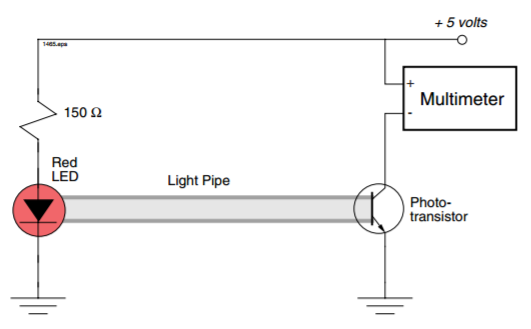
\includegraphics[scale=0.7]{circuit.png}
	\caption{Our circuit for this lab}
\end{figure}
\item We measured the difference with the LED on or off (by removing it from the circuit) with:
	\begin{itemize}
	\item Ambient light
	\item A light tube connecting the LED and phototransistor
	\item A light tube filled with water connecting the LED and phototransistor
	\item A light tube filled with water connecting the LED and phototransistor, with a 90 degree bend
	\end{itemize}
\item We then removed the light tube and replaced it with a commercial waveguide, additionally covering the photoresist so only the light through the waveguide affects the photoresist. This was done using:
	\begin{itemize}
	\item Green light
	\item Red light
	\item Infrared light
	\end{itemize}
This needed to be done multiple times for differing waveguide lengths but time constraints only allowed our group to take one trial at each green light, red light, and IR. 

\textit{Roshan Plamthottam's data which consists of two waveguide lengths and extrapolated data was used instead.}
\end{itemize}
\subsubsection*{Lab 2c solutions}
\begin{itemize}
\item We prepared 6 solutions of DI water, chlorobenzene, bromobenzene, C Cl4, toluene, and octane.
\item We prepared 6 samples of large soda lime ash(glass), smaller soda lime ash, acrylamide beads, acrylamide beads swollen with water, borosilicate glass, and polystyrene beads.
\item We placed samples one at a time into each solution, ranking the observed visibility of each sample on a scale from 1-6, with a rating of 1 denoting completely visible substances and 6 denoting invisibility.
\end{itemize}

\section*{Results and Discussion}
\subsubsection*{Lab 2a}
\ \ \ The results of Lab 2a are shown below in \textbf{Figure 6}, converting 3 measurements at each point to an average value. The critical equation used for this graph was \textbf{Equation 4}. We plot capacitance on the y axis, and $\varepsilon_0\frac{A}{D}$ on the x axis. Thus, the slope of each line is $\varepsilon_r$, the dielectric constant. The data points were taken at 100Hz, then 1kHz, then 100kHz, shown below in \textbf{Figure 6}. Here, the grey is firebrick, the orange is glass, and the blue is ceramic.

\begin{figure}[h!]
	\centering
	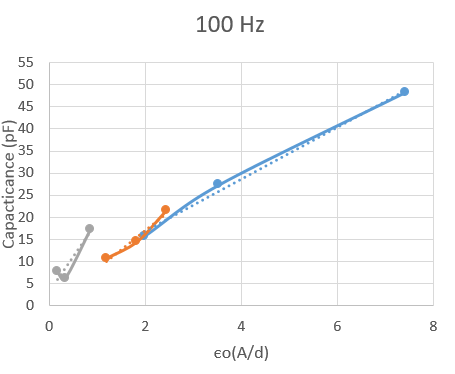
\includegraphics[scale=0.9]{100.png}\\
	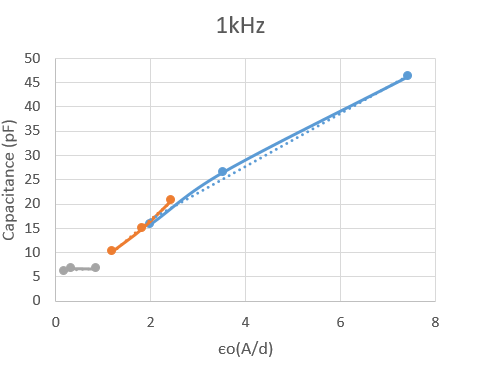
\includegraphics[scale=0.92]{1k.png}\\
	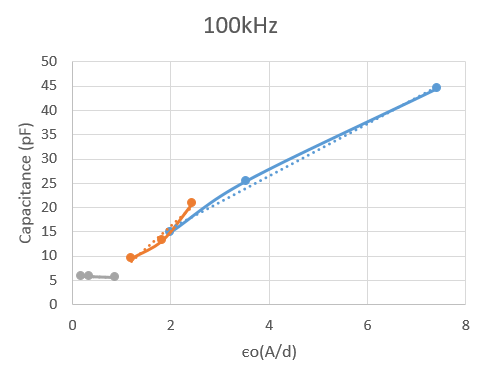
\includegraphics[scale=0.87]{100k.png}
	\caption{Capacitance measurements of 3 materials at 100Hz, 1kHz, and 100Hz}
\end{figure}

The values of dieletric constants for cermaic were 5.87, 5.49, and 5.37 for 100, 1k, and 100k Hz respectively. The values of dieletric constants for Glass were 8.71, 8.62, and 9.16. The values of dieletric constants for Firebrick were 15.81, 0.62, and -0.18. Analysis of these results is assisted by an understanding of \textbf{Figure 3}. However, this figure is just a general trend and differs for each material, so we cannot make firm conclusions simply from this figure. One must still keep in mind that since many different behaviors are possible, we should operate under the assumption that the observed trends may be affected from error in the experiment. In other words, the observed increasing trend from glass could  be due to a combination of the predicted behavior and the random error in the measurements. This is seen more clearly in the firebrick data, since dielectric constants less that 1 are not physically possible from \textbf{Equation 3}.\\

Our verification of the capacitance equatoin, \textbf{Equation 4}, is done by observing the linearity of our regression lines. The $r^2$ value measures how closely our plot resembles lines - where a 1.0 shows perfect linearity. These $r^2$ values, in this case at 100Hz, are 0.9937 for ceramic, 0.9664 for glass, and 0.8865 for firebrick. This reflects what we have been seeing in terms of expected error in our measurements.\\

From \textbf{Figures 3 and 6}, it seems clear that the ceramic material is in a state of decay of one of its polarization types. The glass material, then, could be in one of the regions with increased interaction of a specific polarization where one can observe an increase in dielectric constant. The other possibility is that our error simply masked a similar decay of dielectric, which seems more likely due to the large range of frequencies measured. The firebrick data is clearly incorrect since its capacitance values are impossible, but we see a decreasing trend that we expect from loss of polarization types.\\

The systematic error source from the LCR machine can be assumed to be negligible when compared to other error. However, we also have an error source from our firebrick sample. This is due to the nature of the material, and is clearly systematic due to the persistent high error we see with our firebrick data in labs 2a and 2b. The random error in this part of the lab is due to the strength of connections in our LCR circuit varying randomly as well as which value we randomly decide to report.\\

Comparing our dielectric constants to literature values of 9.8 for ceramic(alumina), 4.6 for glass, and 6.1 for firebrick gives predictable results considering our error. Our average dielectrics across all frequencies are 5.58 for ceramic, 8.83 for glass, and 5.41 for firebrick. An interesting point to note is that our only material which is transparent, glass, has a higher dielectric constant than our other two materials. This implies that the behavior of photons passing through a material is proportional to its polarizability, which makes sense.

\subsubsection*{Lab 2b}
\ \ \ Lab 2b data, as mentioned in the procedure, was mistakenly only used at three different frequencies. Since we needed five, we used Maria Lugo's group's data. The analysis of this data does not include a verification of the capacitance equation. However, we compare the general trend shown in \textbf{Figure 3} more closely since we have 5 different measurements for each frequency.

\begin{figure}[h!]
	\centering
	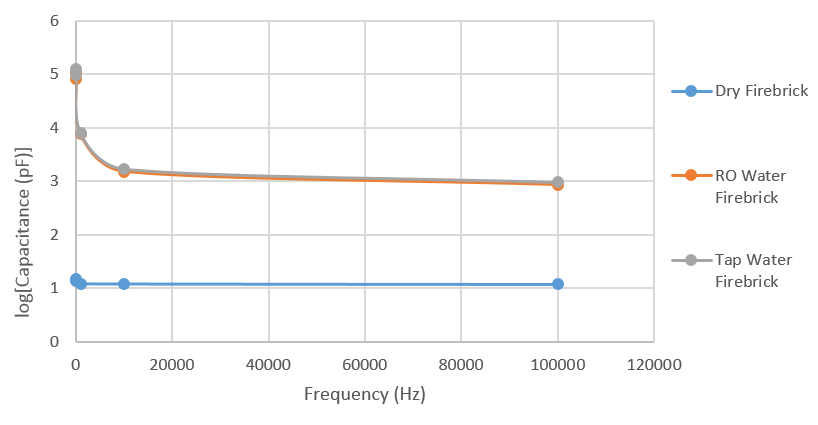
\includegraphics[scale=0.775]{2b.png}
	\caption{Capacitance measurements of firebrick at 5 different frequencies}
\end{figure}

The decrease in capacitance as we increase frequency is predicted as we predicted. Additionally, we can analyze the predicted capacitance changes as we add charge carriers to the firebrick. The addition of charge carriers, observed in \textbf{Figure 2}, is the ionic polarization. This is because tap water contains ions in the form of certain ion concentrations. RO water also has charge carriers, but fewer. Noticeably small differences are seen between the RO water and tap water, though there still was one. This is likely due to the fact that, although RO water has no ion concentrations of other particles, there is still a natural distribution of hydronium and hydroxide ions that naturally form in water that act as charge carriers even if it is RO water.\\

The error sources are similar to lab 2a, except for a few key differences. The biggest error source from this lab from what was expected was systematic - we used ro water instead of DI water. This main difference meant that the number of charge carriers is significantly higher in ro water when compared to DI water. The result was that the tap water's capacitance was much closer to the second curve of our ro water capacitance.

\subsubsection*{Lab 2c, circuit}
\ \ \ Our Lab2c circuit data was all correct except for the last section since we only measured one length of waveguide. Thus, we used Roshan Plamthottam's group's data for that part.

For the first part of the lab, we set up our LEDs and our circuit as shown in the procedure. Our circuit measurement comparisons are shown below in \textbf{Figure 8}.

\begin{figure}[h!]
	\centering
	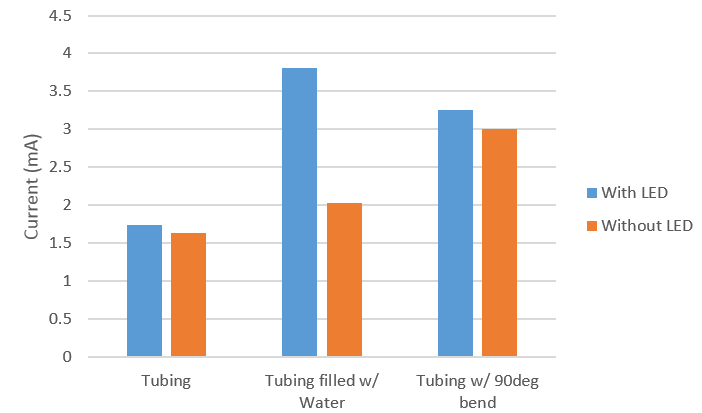
\includegraphics[scale=0.77]{bar.png}
	\caption{Comparing current with a phototransistor with different environments}
\end{figure}

The above figure has 3 pairs of data with the red LED either turned on or off. The first pair was with an air column inside vinyl tubing connecting the LED to the phototransistor. Here, the ambient light in the room allowed current to flow. The impact of the LED can be determined by the difference in values between the two bars in each pair. It is an indicator of how effective our light tube is. The first pair shows negligible LED impact. The second pair, with water in our tubing, has a more pronounced difference between LED modes. This difference can be explained by an improvement in the light tube due to a more optimal water-vinyl refractory interface. This is a result of \textbf{Equation 7}, Snell's law - water has a higher refractive index than air. The third pair of bars shows water-filled light tubing with a bend. This bend is significant visually as we see that the LED impact has been reduced once again. This can be attributed once more to \textbf{Equation 7}, since part of Snell's law depends on the incident angle of the beam. In normal conditions, slight curvature in a light tube will be able to totally internally reflect the beam. However, in more extreme circumstances such as a sharp bend, the interface will not refract the light enough and signal will be lost. The next experiment done was, as mentioned above, done only at one length, so we used another group's data.

\begin{figure}[h!]
	\centering
	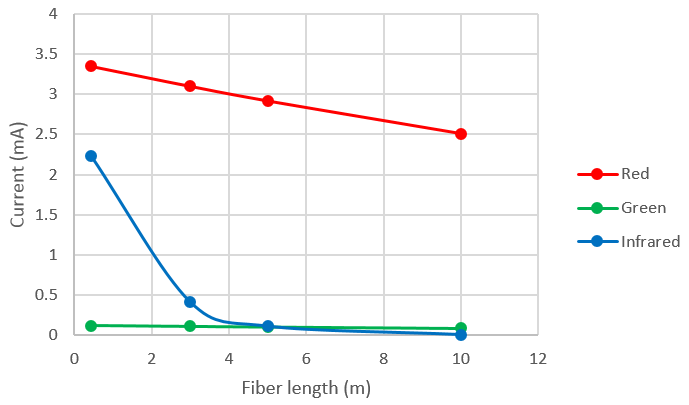
\includegraphics[scale=0.77]{2c.png}
	\caption{Current for different lights with waveguides}
\end{figure}

The trends shown in \textbf{Figure 9} follow the correct pattern that we predicted in the introduction with \textbf{Equations 8, 9, and 10}. The optical fiber transmits specific wavelengths better than others. The specific value of our data is not as relevant as the slopes. From \textbf{Figure 9}, we see that the plastic optical fiber we used is not designed to transmit infrared light as the current dropped significantly as length increased. This implies that the light transmitted also dropped.\\

\subsubsection*{Questions}
In order to find the power, we simply multiply current by voltage using the equation $P = IV$.\\
\textit{Water in the core}\\
Current = 1.7366mA
$$\frac{1.7366mA}{1} * \frac{1mW}{50mA} = 0.0347mW$$
\textit{No water in the core}\\
Current = 3.81mA
$$\frac{3.81mA}{1} * \frac{1mW}{50mA} = 0.0762mW$$
\ \ \ The attenuation factor for red and green like are about the same but the attenuation factor for infrared light is approximately twice as large. The larger attenuation factor means the light beam is attenuated (weakened) more readily which makes sense because IR waves are lower in energy than visible light waves. The tables that we generated for the rest of the questions are in the appendix, numbered \textbf{2, 3, 4, and 5}. \textbf{Table 2} described the attentation coefficient $\alpha$ using \textbf{Equation 10}. \textbf{Table 3} found $P_0$, the launch power, with \textbf{Equation 8}. \textbf{Table 4} used the same equation as 3 but with a 5 meter fiber length. \textbf{Table 5} did the same but with a 10 meter fiber length.\\

In this lab experiment error can be attributed to a number of factors. Because the measurements read by the photo transistor are heavily dependent on the light that the transistor receives there is a great deal of random error associate with the ambient light environment. For example, shadows cast from our lab members’ hands could influence the light reaching the photoresist. Additionally the 90 degree bends was only approximately made by hand so there will be uncertainty in the measurements associated with those calculations. Furthermore, there is no way to ensure how much light is lost by the LED emitter from trial to trial due to the different orientation of the vinyl light guide or the waveguide. As for systematic error there was very little systematic error that can be attributed to anything other than our instruments. The strength and positioning of the connections in our circuit may have subjected our readings to potential deviations from true current readings. Perhaps data bias or poor measurements in the ammeter or photo transistor could contribute to the systematic error. It is important to note that between the trials with the vinyl light guide and the waveguide our photo transistor stopped function and was exchanged for a different one which also will contribute to error in ammeter measurements. 

\subsubsection*{Lab 2c, index of refraction}
\ \ \ This part of the lab was less calculation-intensive than the previous parts since our measurements were all qualitative and the goal was to simply find a trend. However, some quantification is necessary, which is possible if one looks up the literature values of the indices of refraction of all our solvents and samples. The quantitative measurements are shown in the appendix in \textbf{Table 1}. This follows the general trend of our visual rankings in \textbf{Figure 10} below.

\begin{figure}[h!]
\ \ \ \ \ \ \ \ \ \ \ \ \ \ \ \ \ \ \ \ \ \ 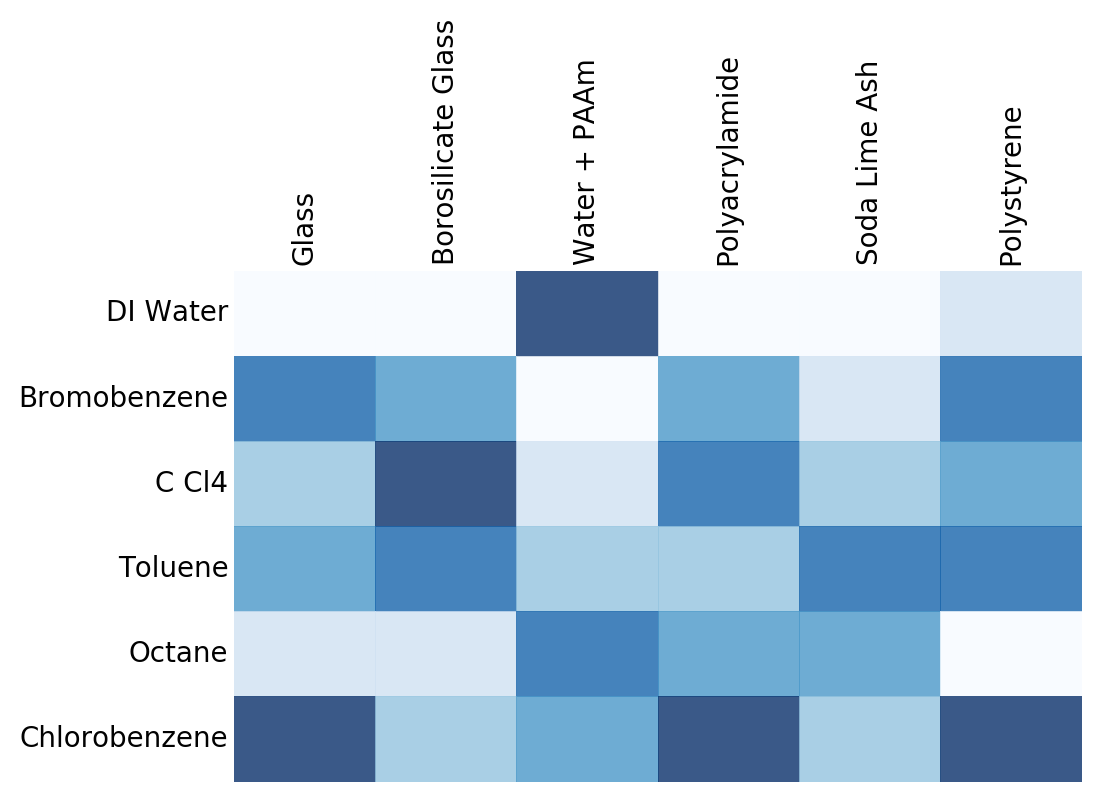
\includegraphics[scale=0.35]{boi.png}
	\caption{A heatmap, darker blue colors represent more invisibility}
\end{figure}

The literature values for our materials were found with \textbf{References 1 and 2}.\\

It is clear that our values indicating almost perfect invisibility are due to  low differences in the index of refraction. These values reflect the relationship given by Snell's Law in \textbf{Equation 7}. Interesting conclusions that can be drawn from this part of the lab is how different properties of a material will affect how light refracts off of it. For example, a hydrogel that absorbs water will have its index of refraction changed closer to water the more water it absorbs, seen in \textbf{Figure 9} between row one column 3 and row one column four. Additionally, the sizes of the particles affects how we visually perceive invisibility since many small particles have more interfaces which are more visible, as seen in the differences in values between column 1 and column 5. These two columns are similar materials with different radii, changing the incident ray angle and affecting how visible the particles were.\\

Error in this part of the lab is partially from chemical reaction between the sample and solvent interfering with the visibility - a systematic error. Additionally, random error was created when we visually compared the visibilities of different materials since they had very similar visibilities in some cases.

\clearpage
\section*{Appendix}
\subsubsection*{Data Tables}
\begin{table}[h!]
	\centering
	\begin{tabular}{| c | c | c |}
	\hline
	Material & Closest Solvent & \% deviation of RI\\
	\hline
	\hline
	Glass(multipurpose) & Chlorobenzene & 0.02\%\\
	\hline
	Borosilicate glass & $C Cl_4$ & 3.76\%\\
	\hline
	Water+PAAm & DI water & 0.00\%\\
	\hline
	PAAm & Chlorobenzene & 5.01\%\\
	\hline
	Soda lime ash & Toluene & 1.74\%\\
	\hline
	Polystyrene & Chlorobenzene & 1.86\%\\
	\hline
	\end{tabular}
	\caption{Refractive Index Deviations}
\end{table}
\begin{table}[h!]
\centering
\includegraphics[scale=1.2]{{Act3_Table3.2}.png}
\caption{Hm}
\end{table}
\begin{table}[h!]
\centering
\includegraphics[scale=1.2]{{Act3_Table3.3}.png}
\caption{Hm}
\end{table}
\begin{table}[h!]
\centering
\includegraphics[scale=1.2]{{Act3_Table3.4}.png}
\caption{Hm}
\end{table}
\begin{table}[h!]
\centering
\includegraphics[scale=1.2]{{Act3_Table3.5}.png}
\caption{Hm}
\end{table}
\subsubsection*{References}
\subsubsection*{1}
"Polyacrylamide Solution 434930." Sigma-Aldrich. N.p., n.d. Web. 13 Mar. 2017.
\subsubsection*{2}
"Optical Constants of Soda Lime GlassRubin 1985: Clear; N,k 0.31-4.6 µm." Refractive Index of Soda Lime Glass - Rubin-clear. N.p., n.d. Web. 13 Mar. 2017.
\subsubsection*{3}
Introduction:
Callister, William D. “Electronic Properties.” Materials Science and Engineering: An Introduction. New York: John Wiley \& Sons, 2007. 665-715. Print.    
\subsubsection*{4}
"Electromagnetic Radiation." Electromagnetic Radiation. University of Oregon, n.d. Web. 13 Mar. 2017.

\end{document}